\thispagestyle{plain}

\section{Data}

The data used was  the \href{https://www.kaggle.com/rmisra/news-headlines-dataset-for-sarcasm-detection}{\color{blue}{News Headlines Dataset For Sarcasm Detection}}\citep{misra2019sarcasm} found on Kaggle.  This dataset consists of news headlines from two different websites: \href{https://www.theonion.com}{\color{blue}{The Onion}}, a satiric news website where all headlines and articles are sarcastic/humorous, and \href{https://www.huffpost.com}{\color{blue}{Huffpost}}, a real news website where its headlines are considered 'not sarcastic'. It is clear that there is a difference in tone and language when it comes to these websites, as evidenced in Figure~\ref{fig-huff} and~\ref{fig-onion}. 

\begin{figure}[!htb]
	\centering
	\subfloat[]{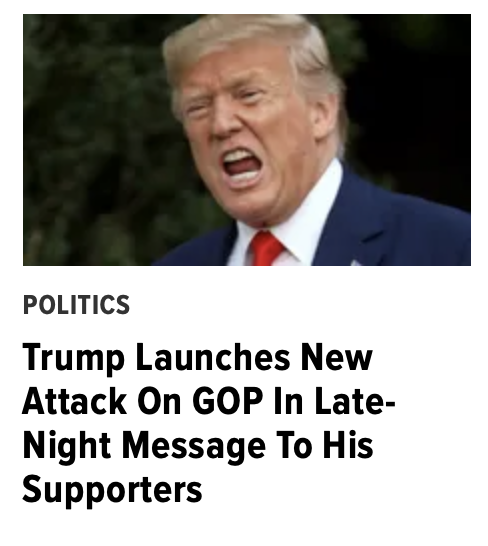
\includegraphics[width=0.43\textwidth]{../img/huffpost.png}\label{fig-huff}}
	\hfill
	\subfloat[]{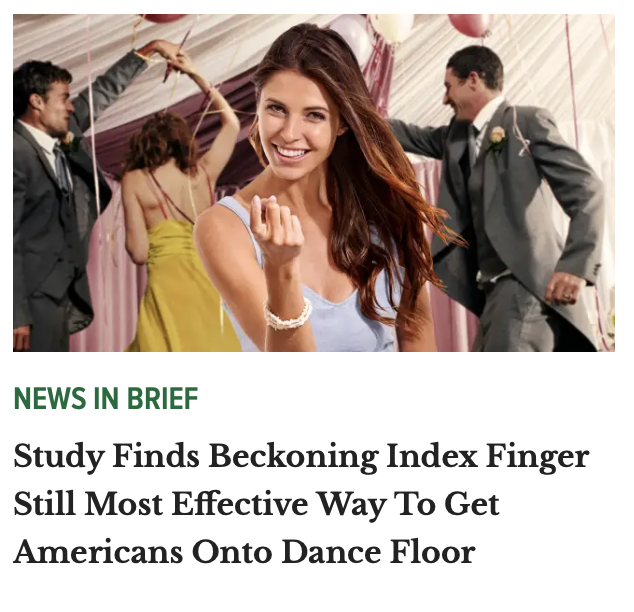
\includegraphics[width=0.5\textwidth]{../img/the-onion.png}\label{fig-onion}}
	\caption{Sample of (a) not sarcastic and (b) sarcastic headlines from Huffpost and The Onion.}
\end{figure}

The raw data is in JSON format and contains information on 28619 headlines. The fields available are:

\begin{itemize}
	\itemsep0em 
	\item{is\_sarcastic: Boolean.Wheter the headline is sarcastic or not.}
	\item{headline: String. Headline text.}
	\item{article\_link: String. URL pointing to the headline's article.}
\end{itemize}

The analysis of this report is focused on the headline text and its class. The article link, therefore, is discarded. Apart from that, no further preprocessing was done.

The classes were found to be fairly balanced, as shown in Figure~\ref{counts} and ~\ref{freq}: 14985 non-sarcastic headlines against 13634 sarcastic ones, that is 52,36\% and 47,64\% of the total headlines respectively. A sample of the dataset is available in Table ~\ref{table:sample}.

\begin{figure}[!tbp]
	\centering
	\subfloat[]{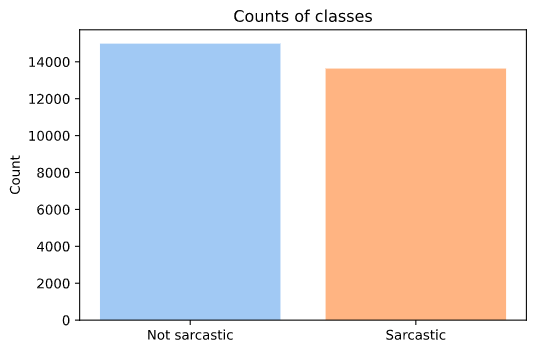
\includegraphics[width=0.5\textwidth]{../img/counts.png}\label{counts}}
	\hfill
	\subfloat[]{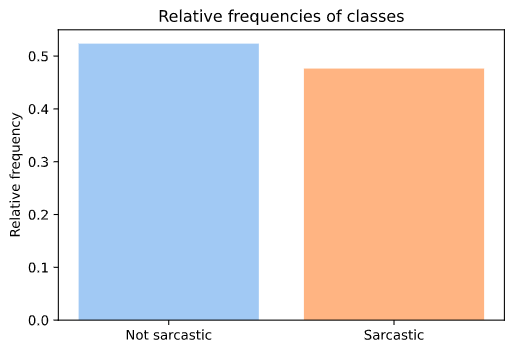
\includegraphics[width=0.48\textwidth]{../img/freq.png}\label{freq}}
	\label{class-balance}
	\caption{(a) Absolute count and (b) Relative frequencies of classes.}
\end{figure}

\newpage
\begin{longtable}[]{p{12cm}lp{}}
	\toprule
	Text & Label \tabularnewline
	\midrule
	\endhead
	'thirtysomething scientists unveil doomsday clock of hair loss'  & 1 \\ \tabularnewline
	
	'dem rep. totally nails why congress is falling short on gender, racial equality' & 0 \\ \tabularnewline
	
	'eat your veggies: 9 deliciously different recipes' & 0  \\ \tabularnewline
	
	'inclement weather prevents liar from getting to work' & 1\\   \tabularnewline
	
	"mother comes pretty close to using word 'streaming' correctly" & 1 \\ \tabularnewline
	
	'my white inheritance' & 0\\ \tabularnewline
	
	'5 ways to file your taxes with less stress' & 0 \\ \tabularnewline
	
	"richard branson's global-warming donation nearly as much as cost of failed balloon trips" & 1 \tabularnewline

	\bottomrule
	\caption{Sample of final dataset.}
	\label{table:sample}
\end{longtable}





